\documentclass[11pt]{article}
\include{noteinclude}
\usepackage{natbib}

\newcommand\descrip[1]{\textsf{\textbf{\large{#1}}}\\}
\newcommand\Rplan{R$_{\mathrm{plan}}$}

\parindent 0pt


\begin{document}

\begin{center}
\Large \textbf{The MOSTLEE Model}

\large \textbf{A Model Of Sources, Transport, Loss, and Emission in Exospheres}

Dr.\ Matthew H.\ Burger
\end{center}
\normalsize

\vspace{2in}
Last Updated: \today

\clearpage
%%%%%%%%%%%%%%%%%%%%%%%%%%%%%%%%%%%%%%%%%%%%%%%%%%%%%%%%%%%%%%%%%%%%%%%%

\tableofcontents
\listoftables
\listoffigures
\clearpage
%%%%%%%%%%%%%%%%%%%%%%%%%%%%%%%%%%%%%%%%%%%%%%%%%%%%%%%%%%%%%%%%%%%%%%%%

\section{$\checkmark$ AtomicData/get\_gvalue\_3.1.pro} \label{sec:get_gvalue}

\descrip{Summary}
Creates a g-value structure using saved atomic data.

\descrip{Calling Procedure}
\verb+gval = get_gvalue, atom, a, path=path+

\descrip{Inputs}
\begin{compactenum} \listup
\item atom = species being modeled
\item a = heliocentric distance
\item path = path where g-values are saved (optional)
\end{compactenum}

\descrip{Outputs}
Function returns a structure with the fields:
\begin{compactitem}
\item species = same as the atom input
\item a = same as the input. Units: AU.
\item wavelength = pointer to an array of length $nlam$ with wavelengths of 
resonance transitions. Units: \AA.
\item v = pointer to an array of length $nvel$ with the radial velocities at 
which the g-value was calculated Units: km cm$^{-2}$ s$^{-1}$.
\item g = pointer to an array of size $nvel \times nlam$ with g-values as
function of radial velocity for each resonant transition scaled to distance 
$a$ . Units: photons s$^{-1}$. 
\item radaccel = pointer to an array of size $nvel$ with the radiation 
acceleration at each wavelength. See
\hyperref[sec:radiation_pressure]{radiation\_pressure} and
Figure~\ref{fig:radaccel}. Units: km s$^{-1}$.
\item If the species is not found, a warning is printed and the g-value is set
to 0.
\end{compactitem}

\descrip{Model Procedures Called}
None.

\descrip{Notes}
\begin{compactenum}
\item The g-values are saved in \texttt{\$BASEPATH/Work/AtomicData/g-values/'}
\item The structure saved in the g-value files are created with
\texttt{set\_up\_gvals}.
\item See Table~\ref{table:gval} for list of species that have g-values
implemented in the code.
\item Figure~\ref{figure:gval} shows g-value at 1 AU as function of radial 
velocity for each species listed in Table~\ref{table:gval}.
\end{compactenum}

\descrip{This Page Last Updated}
12 December 2011.

\begin{table}[b]
\begin{tabular}{lll}
\textbf{Species} & \textbf{Wavelengths (\AA)} & \textbf{Reference} \\ \hline
C & 1560, 1657 & \citet{killen2009} \\
Ca\plus & 3934, 3969 & \citet{killen2009} \\
Ca & 2722, 4227, 4567 &  \citet{killen2009} \\
H & 1215 &  \citet{killen2009} \\
He & 584 &  \citet{killen2009} \\
K & 4045 &  \citet{killen2009} \\
Mg\plus & 2083, 2796 &  \citet{killen2009} \\
Mg & 2026, 2852, &  \citet{killen2009} \\
Mn & 2795, 2799, 2802 & XXXXX \\
Na & 3303, 5891, 5897 & \citet{killen2009} \\
O & 1303 & \citet{killen2009} \\
OH & 3081, 3092 &  \citet{killen2009} \\
S & 1807, 1820 &  \citet{killen2009} \\
Ti & 3187, 3193, 3204, 3342, 3371, 3371, 3636, 3644 &  XXXXX
\end{tabular}
\caption{Available g-values}
\label{table:gval}
\end{table}

\clearpage
%%%%%%%%%%%%%%%%%%%%%%%%%%%%%%%%%%%%%%%%%%%%%%%%%%%%%%%%%%%%%%%%%%%%%%%%

\section{$\checkmark$Data/SystemConstants\_2.0.pro} \label{sec:systemconstants}

\descrip{Summary} 
Creates the \texttt{SystemConsts} and \texttt{DipoleConsts} structures from 
data stored in the \textit{!consts} system variables.

\descrip{Calling Procedure}
\verb+SystemConstants, planet, SystemConsts, DipoleConsts+

\descrip{Inputs} 
\begin{compactitem} \listup
\item planet: String containing planet name. For purposes of the model,
\textit{planet} is defined as the center of the modeled system.
Therefore, "sun" and "pluto" are valid planets.
\end{compactitem}

\descrip{Outputs}
\begin{compactitem} \listup
\item SystemConsts: Structure containing the planetary system constants
The fields in the structure are given in Table~\ref{table:systemconsts}. The
values for each object are given in Table~\ref{table:systemvalues}.

\item DipoleConsts: Structure containing the planetary dipole constants 
The fields in the structure are given in Table~\ref{table:dipoleconsts}. 
The values for each object are given in Table~\ref{table:systemvalues}.
\end{compactitem}

\descrip{Model Procedures Called}
None.

\descrip{Notes}
\begin{compactenum} \listup
\item The values used in this routine are saved in the files 
\texttt{Data/PhysicalData/PlanetaryConstants.dat} and 
\texttt{Data/PhsyicalData/DipoleConstants.dat}. 
\item Data taken from 
\href{http://ssd.jpl.nasa.gov/?phys_data}{NASA Solar System Dynamics} and 
\href{http://en.wikipedia.org/wiki/Sun}{Wikipedia: Sun}.
\end{compactenum}

\descrip{This Page Last Updated}
9 December 2011.


\clearpage
%%%%%%%%%%%%%%%%%%%%%%%%%%%%%%%%%%%%%%%%%%%%%%%%%%%%%%%%%%%%%%%%%%%%%%%%

\section{$\checkmark$Display/determine\_image\_rotation\_4.0.pro}
\label{sec:determine_image_rotation}

\descrip{Summary}

Computes the rotation matrix for an image given a sub-observer longitude, 
sub-observer latitude, and
north pole rotation angle, or a time and observer location.

\descrip{Calling Procedure}

\verb+M = determine_image_rotation, input, format+

\descrip{Inputs}
\begin{compactenum} \listup
\item input = input structure
\item format = format structure
\end{compactenum}

\descrip{Outputs}
Returns the rotation matrix from model coordinates to the observer's viewpoint.

\descrip{Model Procedures Called}
\begin{compactenum} \listup
\item \texttt{relative\_position}
\item \texttt{utc2et}
\item \texttt{rotationmatrix}
\item \texttt{rotation}
\end{compactenum}

\descrip{Notes}
\begin{compactenum} \listup
\item There are two ways to specify the observing geometry:
  \begin{compactenum} 
  \item Sub-Observer point:
    \begin{compactitem}
    \item format.geometry.SubObsLongitude: radians dawnward of sub-solar point
    \item format.geometry.SubObsLatitude: radians northward of sub-solar point
    \item format.geometry.PolarAngle: north pole rotation angle radians 
    counter-clockwise (?) from north.
    \end{compactitem}
  \item Time and Observer location:
    \begin{compactitem}
    \item format.geometry.time: string time in ISOC format 
    (YYYY-MM-DDTHH:MM:SS.S or YYY-DOYTHH:MM:SS.S)
    \item format.geometry.observer: NAIF observer location (e.g., `Earth', 
    `MESSENGER')
    \end{compactitem}
  \end{compactenum}
  \item The rotation matrix is determined by the rotation angle ($\theta$) of 
  the sun direction ($\mathbf{\hat{x}}_{\astrosun}$) to the observer direction
  ($\mathbf{\hat{x}}_{obs}$) around the axis perpendicular to 
  both vectors ($\mathbf{\hat{a}}$):
    \begin{eqnarray}
    \mathbf{\hat{a}} & = & \mathbf{\hat{x}}_{\astrosun} \times 
      \mathbf{\hat{x}}_{obs} \\
    \cos \theta & = & \mathbf{\hat{x}_{\astrosun}} \cdot \mathbf{\hat{x}}_{obs}
      \\
    M & = & \left( \begin{array}{ccc}
      a_x^2 + (1-a_x)^2 \cos \theta & 
      a_x a_y (1-\cos \theta)-a_z \sin \theta & 
      a_x a_z (1-\cos \theta)+a_y \sin \theta \\

      a_x a_y (1-\cos \theta) + a_z \sin \theta & 
      a_y^2 + (1-a_y^2) \cos \theta & 
      a_y a_z (1-\cos \theta) - a_x \sin \theta \\

      a_x a_z (1-\cos \theta) - a_y \sin \theta & 
      a_y a_z (1-\cos \theta) + a_x \sin \theta & 
      a_z^2 + (1-a_z^2) \cos \theta
      \end{array} \right)
    \end{eqnarray}
  \item If specifying Sub-Observer point, then:
    \begin{eqnarray}
    \mathbf{\hat{x}}_{\astrosun} & = & (0,-1,0) \\
    \mathbf{\hat{x}}_{obs} & = & (\sin \lambda \cos \mu, -cos \lambda \cos \mu,
      \sin \mu)
    \end{eqnarray}
    where $\lambda = $ \textit{input.geometry.SubObsLongitude} and $\mu =$
    \textit{input.geometry.SubObsLatitude}
  \item If specifying Time and Observer location, then
  $\mathbf{\hat{x}}_{\astrosun}$ and $\mathbf{\hat{x}}_{obs}$ are determined
  with \texttt{relative\_position} using SPICE.
  \item If \textit{format.geometry.PolarAngle} $\neq 0$, then a rotation is
  taken around the new y-axis.
\end{compactenum}

\descrip{This Page Last Updated}
13 December 2011.

\clearpage
%%%%%%%%%%%%%%%%%%%%%%%%%%%%%%%%%%%%%%%%%%%%%%%%%%%%%%%%%%%%%%%%%%%%%%%%

\section{Display/display\_hull.pro} \label{sec:display_hull}

\descrip{Summary}

\descrip{Calling Procedure}

\descrip{Inputs}

\descrip{Outputs}

\descrip{Model Procedures Called}

\descrip{Notes}

\descrip{This Page Last Updated}

\clearpage
%%%%%%%%%%%%%%%%%%%%%%%%%%%%%%%%%%%%%%%%%%%%%%%%%%%%%%%%%%%%%%%%%%%%%%%%

\section{Display/display\_model\_image\_4.0.pro} \label{sec:display_model_image}

\descrip{Summary}

\descrip{Calling Procedure}

\descrip{Inputs}

\descrip{Outputs}

\descrip{Model Procedures Called}

\descrip{Notes}

\descrip{This Page Last Updated}

\clearpage
%%%%%%%%%%%%%%%%%%%%%%%%%%%%%%%%%%%%%%%%%%%%%%%%%%%%%%%%%%%%%%%%%%%%%%%%

\section{Display/emission\_measure\_2.0.pro} \label{sec:emission_measure}

\descrip{Summary}

\descrip{Calling Procedure}

\descrip{Inputs}

\descrip{Outputs}

\descrip{Model Procedures Called}

\descrip{Notes}

\descrip{This Page Last Updated}

\clearpage
%%%%%%%%%%%%%%%%%%%%%%%%%%%%%%%%%%%%%%%%%%%%%%%%%%%%%%%%%%%%%%%%%%%%%%%%

\section{Display/model\_view.pro} \label{sec:model_view}

\descrip{Summary}

\descrip{Calling Procedure}

\descrip{Inputs}

\descrip{Outputs}

\descrip{Model Procedures Called}

\descrip{Notes}

\descrip{This Page Last Updated}

\clearpage
%%%%%%%%%%%%%%%%%%%%%%%%%%%%%%%%%%%%%%%%%%%%%%%%%%%%%%%%%%%%%%%%%%%%%%%%

\section{Display/produce\_density\_4.1.pro} \label{sec:produce_density}

\descrip{Summary}

\descrip{Calling Procedure}

\descrip{Inputs}

\descrip{Outputs}

\descrip{Model Procedures Called}

\descrip{Notes}

\descrip{This Page Last Updated}

\clearpage
%%%%%%%%%%%%%%%%%%%%%%%%%%%%%%%%%%%%%%%%%%%%%%%%%%%%%%%%%%%%%%%%%%%%%%%%

\section{Display/produce\_image\_4.0.pro} \label{sec:produce_image}

\descrip{Summary}

\descrip{Calling Procedure}

\descrip{Inputs}

\descrip{Outputs}

\descrip{Model Procedures Called}

\descrip{Notes}

\descrip{This Page Last Updated}

\clearpage
%%%%%%%%%%%%%%%%%%%%%%%%%%%%%%%%%%%%%%%%%%%%%%%%%%%%%%%%%%%%%%%%%%%%%%%%

\section{Display/produce\_los\_4.12.pro} \label{sec:produce_los}

\descrip{Summary}

\descrip{Calling Procedure}

\descrip{Inputs}

\descrip{Outputs}

\descrip{Model Procedures Called}

\descrip{Notes}

\descrip{This Page Last Updated}

\clearpage
%%%%%%%%%%%%%%%%%%%%%%%%%%%%%%%%%%%%%%%%%%%%%%%%%%%%%%%%%%%%%%%%%%%%%%%%

\section{Display/produce\_results\_4.1.pro} \label{sec:produce_results}

\descrip{Summary}

\descrip{Calling Procedure}

\descrip{Inputs}

\descrip{Outputs}

\descrip{Model Procedures Called}

\descrip{Notes}

\descrip{This Page Last Updated}

\clearpage
%%%%%%%%%%%%%%%%%%%%%%%%%%%%%%%%%%%%%%%%%%%%%%%%%%%%%%%%%%%%%%%%%%%%%%%%

\section{Display/produce\_voronoi\_image\_4.3.pro}
\label{sec:produce_voronoi_image}

\descrip{Summary}

\descrip{Calling Procedure}

\descrip{Inputs}

\descrip{Outputs}

\descrip{Model Procedures Called}

\descrip{Notes}

\descrip{This Page Last Updated}

\clearpage
%%%%%%%%%%%%%%%%%%%%%%%%%%%%%%%%%%%%%%%%%%%%%%%%%%%%%%%%%%%%%%%%%%%%%%%%

\section{Display/quick\_look.pro} \label{sec:quick_look}

\descrip{Summary}

\descrip{Calling Procedure}

\descrip{Inputs}

\descrip{Outputs}

\descrip{Model Procedures Called}

\descrip{Notes}

\descrip{This Page Last Updated}

\clearpage
%%%%%%%%%%%%%%%%%%%%%%%%%%%%%%%%%%%%%%%%%%%%%%%%%%%%%%%%%%%%%%%%%%%%%%%%

\section{Display/read\_resultformat\_4.2.pro} \label{sec:read_resultformat}

\descrip{Summary}

\descrip{Calling Procedure}

\descrip{Inputs}

\descrip{Outputs}

\descrip{Model Procedures Called}

\descrip{Notes}

\descrip{This Page Last Updated}

\clearpage
%%%%%%%%%%%%%%%%%%%%%%%%%%%%%%%%%%%%%%%%%%%%%%%%%%%%%%%%%%%%%%%%%%%%%%%%

\section{Display/results\_common\_4.0.pro} \label{sec:results_common}

\descrip{Summary}

\descrip{Calling Procedure}

\descrip{Inputs}

\descrip{Outputs}

\descrip{Model Procedures Called}

\descrip{Notes}

\descrip{This Page Last Updated}

\clearpage
%%%%%%%%%%%%%%%%%%%%%%%%%%%%%%%%%%%%%%%%%%%%%%%%%%%%%%%%%%%%%%%%%%%%%%%%

\section{Display/results\_density\_4.5.pro} \label{sec:results_density}

\descrip{Summary}

\descrip{Calling Procedure}

\descrip{Inputs}

\descrip{Outputs}

\descrip{Model Procedures Called}

\descrip{Notes}

\descrip{This Page Last Updated}

\clearpage
%%%%%%%%%%%%%%%%%%%%%%%%%%%%%%%%%%%%%%%%%%%%%%%%%%%%%%%%%%%%%%%%%%%%%%%%

\section{Display/results\_functions\_4.0.pro} \label{sec:results_functions}

\descrip{Summary}

\descrip{Calling Procedure}

\descrip{Inputs}

\descrip{Outputs}

\descrip{Model Procedures Called}

\descrip{Notes}

\descrip{This Page Last Updated}

\clearpage
%%%%%%%%%%%%%%%%%%%%%%%%%%%%%%%%%%%%%%%%%%%%%%%%%%%%%%%%%%%%%%%%%%%%%%%%

\section{Display/results\_kd\_tree\_4.3.pro} \label{sec:results_kd_tree}

\descrip{Summary}

\descrip{Calling Procedure}

\descrip{Inputs}

\descrip{Outputs}

\descrip{Model Procedures Called}

\descrip{Notes}

\descrip{This Page Last Updated}

\clearpage
%%%%%%%%%%%%%%%%%%%%%%%%%%%%%%%%%%%%%%%%%%%%%%%%%%%%%%%%%%%%%%%%%%%%%%%%

\section{Display/results\_packet\_weighting\_4.0.pro}
\label{sec:results_packet_weighting}

\descrip{Summary}

\descrip{Calling Procedure}

\descrip{Inputs}

\descrip{Outputs}

\descrip{Model Procedures Called}

\descrip{Notes}

\descrip{This Page Last Updated}

\clearpage
%%%%%%%%%%%%%%%%%%%%%%%%%%%%%%%%%%%%%%%%%%%%%%%%%%%%%%%%%%%%%%%%%%%%%%%%

\section{Display/results\_voronoi\_4.2.pro} \label{sec:results_voronoi}

\descrip{Summary}

\descrip{Calling Procedure}

\descrip{Inputs}

\descrip{Outputs}

\descrip{Model Procedures Called}

\descrip{Notes}

\descrip{This Page Last Updated}

\clearpage
%%%%%%%%%%%%%%%%%%%%%%%%%%%%%%%%%%%%%%%%%%%%%%%%%%%%%%%%%%%%%%%%%%%%%%%%

\section{$\checkmark$Forces/accel\_3.1.pro} \label{sec:accel}

\descrip{Summary}
Computes the acceleration on a packet due to the specified forces. Possible
forces are gravity, radiation pressure, and Lorentz (not working). 

\descrip{Calling Procedure}
\verb+a = accel(loc, input, magcood, which)+

\descrip{Inputs}
\begin{compactenum} \listup
\item loc = packet location structure
\item input = input structure
\item magcoords = magnetic coordinate structure (which includes
out\_of\_shadow). See \hyperref[sec:xyz_to_magcood]{xyz\_to\_magcoord}.
\item which = array specifying which objects are included in the calculation
\end{compactenum}

\descrip{Outputs}
Function returns a structure with field dvdt, which is an $n\times 3$ array
with $a_x, a_y, a_z$ in units of \Rplan\ s$^{-2}$.

\descrip{Model Procedures Called}
\begin{compactenum} \listup
\item \hyperref[sec:gravity]{gravity}
\item \hyperref[sec:radiation_pressure]{radiation\_pressure}
\item \hyperref[sec:lorentz]{Lorentz}
\end{compactenum}

\descrip{Notes}
\begin{compactenum} \listup
\item Total acceleration:
\begin{equation}
\mathbf{a} = \mathbf{a}_{grav} + \mathbf{a}_{radpres} + \mathbf{a}_{lor}
\end{equation}
\item The input structure fields \texttt{input.Forces.gravity},
\texttt{input.Forces.radpres}, and \texttt{input.Forces.Lorentz} are used to
specify which forces are included in the calculations.
\item The Lorentz force, which only affects ions, does not currently work
properly.
\end{compactenum}

\descrip{This Page Last Updated}
12 December 2011.

\clearpage
%%%%%%%%%%%%%%%%%%%%%%%%%%%%%%%%%%%%%%%%%%%%%%%%%%%%%%%%%%%%%%%%%%%%%%%%

\section{$\checkmark$Forces/gravity\_3.1.pro} \label{sec:gravity}

\descrip{Summary}
Computes acceleration due to gravity from each object.

\descrip{Calling Procedure}
\verb+agrav = gravity(loc, input)+

\descrip{Inputs}
\begin{compactenum} \listup
\item loc = packet location structure
\item input = input structure
\end{compactenum}

\descrip{Outputs}
Function returns acceleration due to gravity as a $n\times3$ array with 
$a_x, a_y, a_z$ in units of \Rplan\ s$^{-2}$.

\descrip{Model Procedures Called}
\begin{compactenum} \listup
\item \hyperref[sec:locmoon]{locmoon}: gives the location of each object as 
viewed by each packet. 
\end{compactenum}

\descrip{Notes}
\begin{compactenum} \listup
\item Gravity computed by:
\begin{eqnarray}
\mathbf{a} & = & \sum_{i=0}^{nobj} \frac{GM}{r_i^2} \mathbf{\hat{r_i}} \\
r_i & = & \sqrt{(x-x_i)^2 + (y-y_i)^2 + (z-z_i)^2}
\end{eqnarray}
which is given in component form by:
\begin{eqnarray}
a_x & = & \sum_{i=0}^{nobj} \frac{GM_i (x-x_i)}{r_i^3} \\
a_y & = & \sum_{i=0}^{nobj} \frac{GM_i (y-y_i)}{r_i^3} \\
a_z & = & \sum_{i=0}^{nobj} \frac{GM_i (z-z_i)}{r_i^3} \\
\end{eqnarray}
where the coordinates of each object (planet and satellites) are
$\mathbf{r_i} = (x_i,y_i,z_i$) are computed by \texttt{locmoon}, $GM_i$ are 
stored in the
\textit{SystemConsts} variable, and the sum is only performed for objects which
\textit{input.geometry.include} = 1. 
\end{compactenum}

\descrip{This Page Last Updated}
12 December 2011

\clearpage
%%%%%%%%%%%%%%%%%%%%%%%%%%%%%%%%%%%%%%%%%%%%%%%%%%%%%%%%%%%%%%%%%%%%%%%%

\section{Forces/lorentz\_2.0.pro} \label{sec:lorentz}

\descrip{Summary}

\descrip{Calling Procedure}

\descrip{Inputs}

\descrip{Outputs}

\descrip{Model Procedures Called}

\descrip{Notes}

\descrip{This Page Last Updated}

\clearpage
%%%%%%%%%%%%%%%%%%%%%%%%%%%%%%%%%%%%%%%%%%%%%%%%%%%%%%%%%%%%%%%%%%%%%%%%

\section{$\checkmark$Forces/radiation\_pressure\_3.1.pro} \label{sec:radiation_pressure}

\descrip{Summary}
Returns the radiation acceleration as function of radial velocity.

\descrip{Calling Procedure}
\verb+radiation_pressure, loc, out_of_shadow+

\descrip{Inputs}
\begin{compactenum} \listup
\item loc = packet location structure
\item out\_of\_shadow = boolean array specifying whether each packet is in the
planet's shadow. \textit{Does not currently compute satellite shadow}
\end{compactenum}

\descrip{Outputs}
Function returns acceleration due to radiation pressure as a $n\times3$ array 
with $a_x, a_y, a_z$ in units of \Rplan\ s$^{-2}$.

\descrip{Model Procedures Called}
None.

\descrip{Notes}
\begin{compactenum}
\item The radiation pressure is computed by:
\begin{equation}
\mathbf{a}_{rad}(v_r) = \sum_i \frac{h g(v_r)}{m \lambda_i} \hat{y}
\end{equation}
where $h=6.6260690\times10^{-27}$ erg s$^{-1}$ is Planck's constant, $g$ is the
g-value as a function of radial velocity relative to the sun $v_r$, $m$ is the
atomic mass, and
$\lambda_i$ is each resonant transition for the species in question.
\item The radiation acceleration is actually calculated by the function
\hyperref[sec:get_gvalue]{get\_gvalue} and stored in the \textit{stuff}
structure in \hyperref[sec:modeldriver]{modeldriver} (in the fields
\textit{stuff.radpres\_v} and \textit{stuff.radpres\_const}). This is done to
speed things up.
\item $\mathbf{a}_{rad}$ is directed entirely in the $+\hat{y}$ direction. I
currently assume the planets' equatorial (rotational) planes are not tilted
relative to their orbital planes.
\item Similarly, $v_{rad}$ is the velocity in the $\hat{y}$ direction (which is
computed relative to the planet) + \textit{stuff.vrplanet}.
\textit{stuff.vrplanet} is computed by \hyperref[sec:planet_dist]{planet\_dist}
and saved into the \textit{stuff} structure in
\hyperref[sec:modeldriver]{modeldriver}.
\item Because the radiation acceleration is computed at discrete values by
\hyperref[sec:get_gvalue]{get\_gvalue}, the radiation acceleration for each
packet is computed by linear interpolation between values.
\item If $v_r$ is outside the velocity range in \textit{stuff.radpres\_v},
then $v_r$ is assumed to be either the maximum or minimum value of
\textit{stuff.radpres\_v}, as appropriate.
\item $\mathbf{a_{rad}} = 0$ in the shadow of a planet or satellite.
\item See Table~\ref{table:gval} for list of species that have g-values
implemented in the code.
\item Figure~\ref{fig:radaccel} shows radiation acceleration as function of
radial velocity at 1 AU for each species listed in Table~\ref{table:gval}.
\end{compactenum}

\descrip{Things to do}
\begin{compactenum} \listup
\item Does not currently compute shadowing for satellites. If radiation
pressure is turned on for a system with multiple objects, program will stop.
\item The radiation acceleration for K is wrong because I do not have the
g-values for the strongest lines.
\end{compactenum}

\begin{figure}[b]
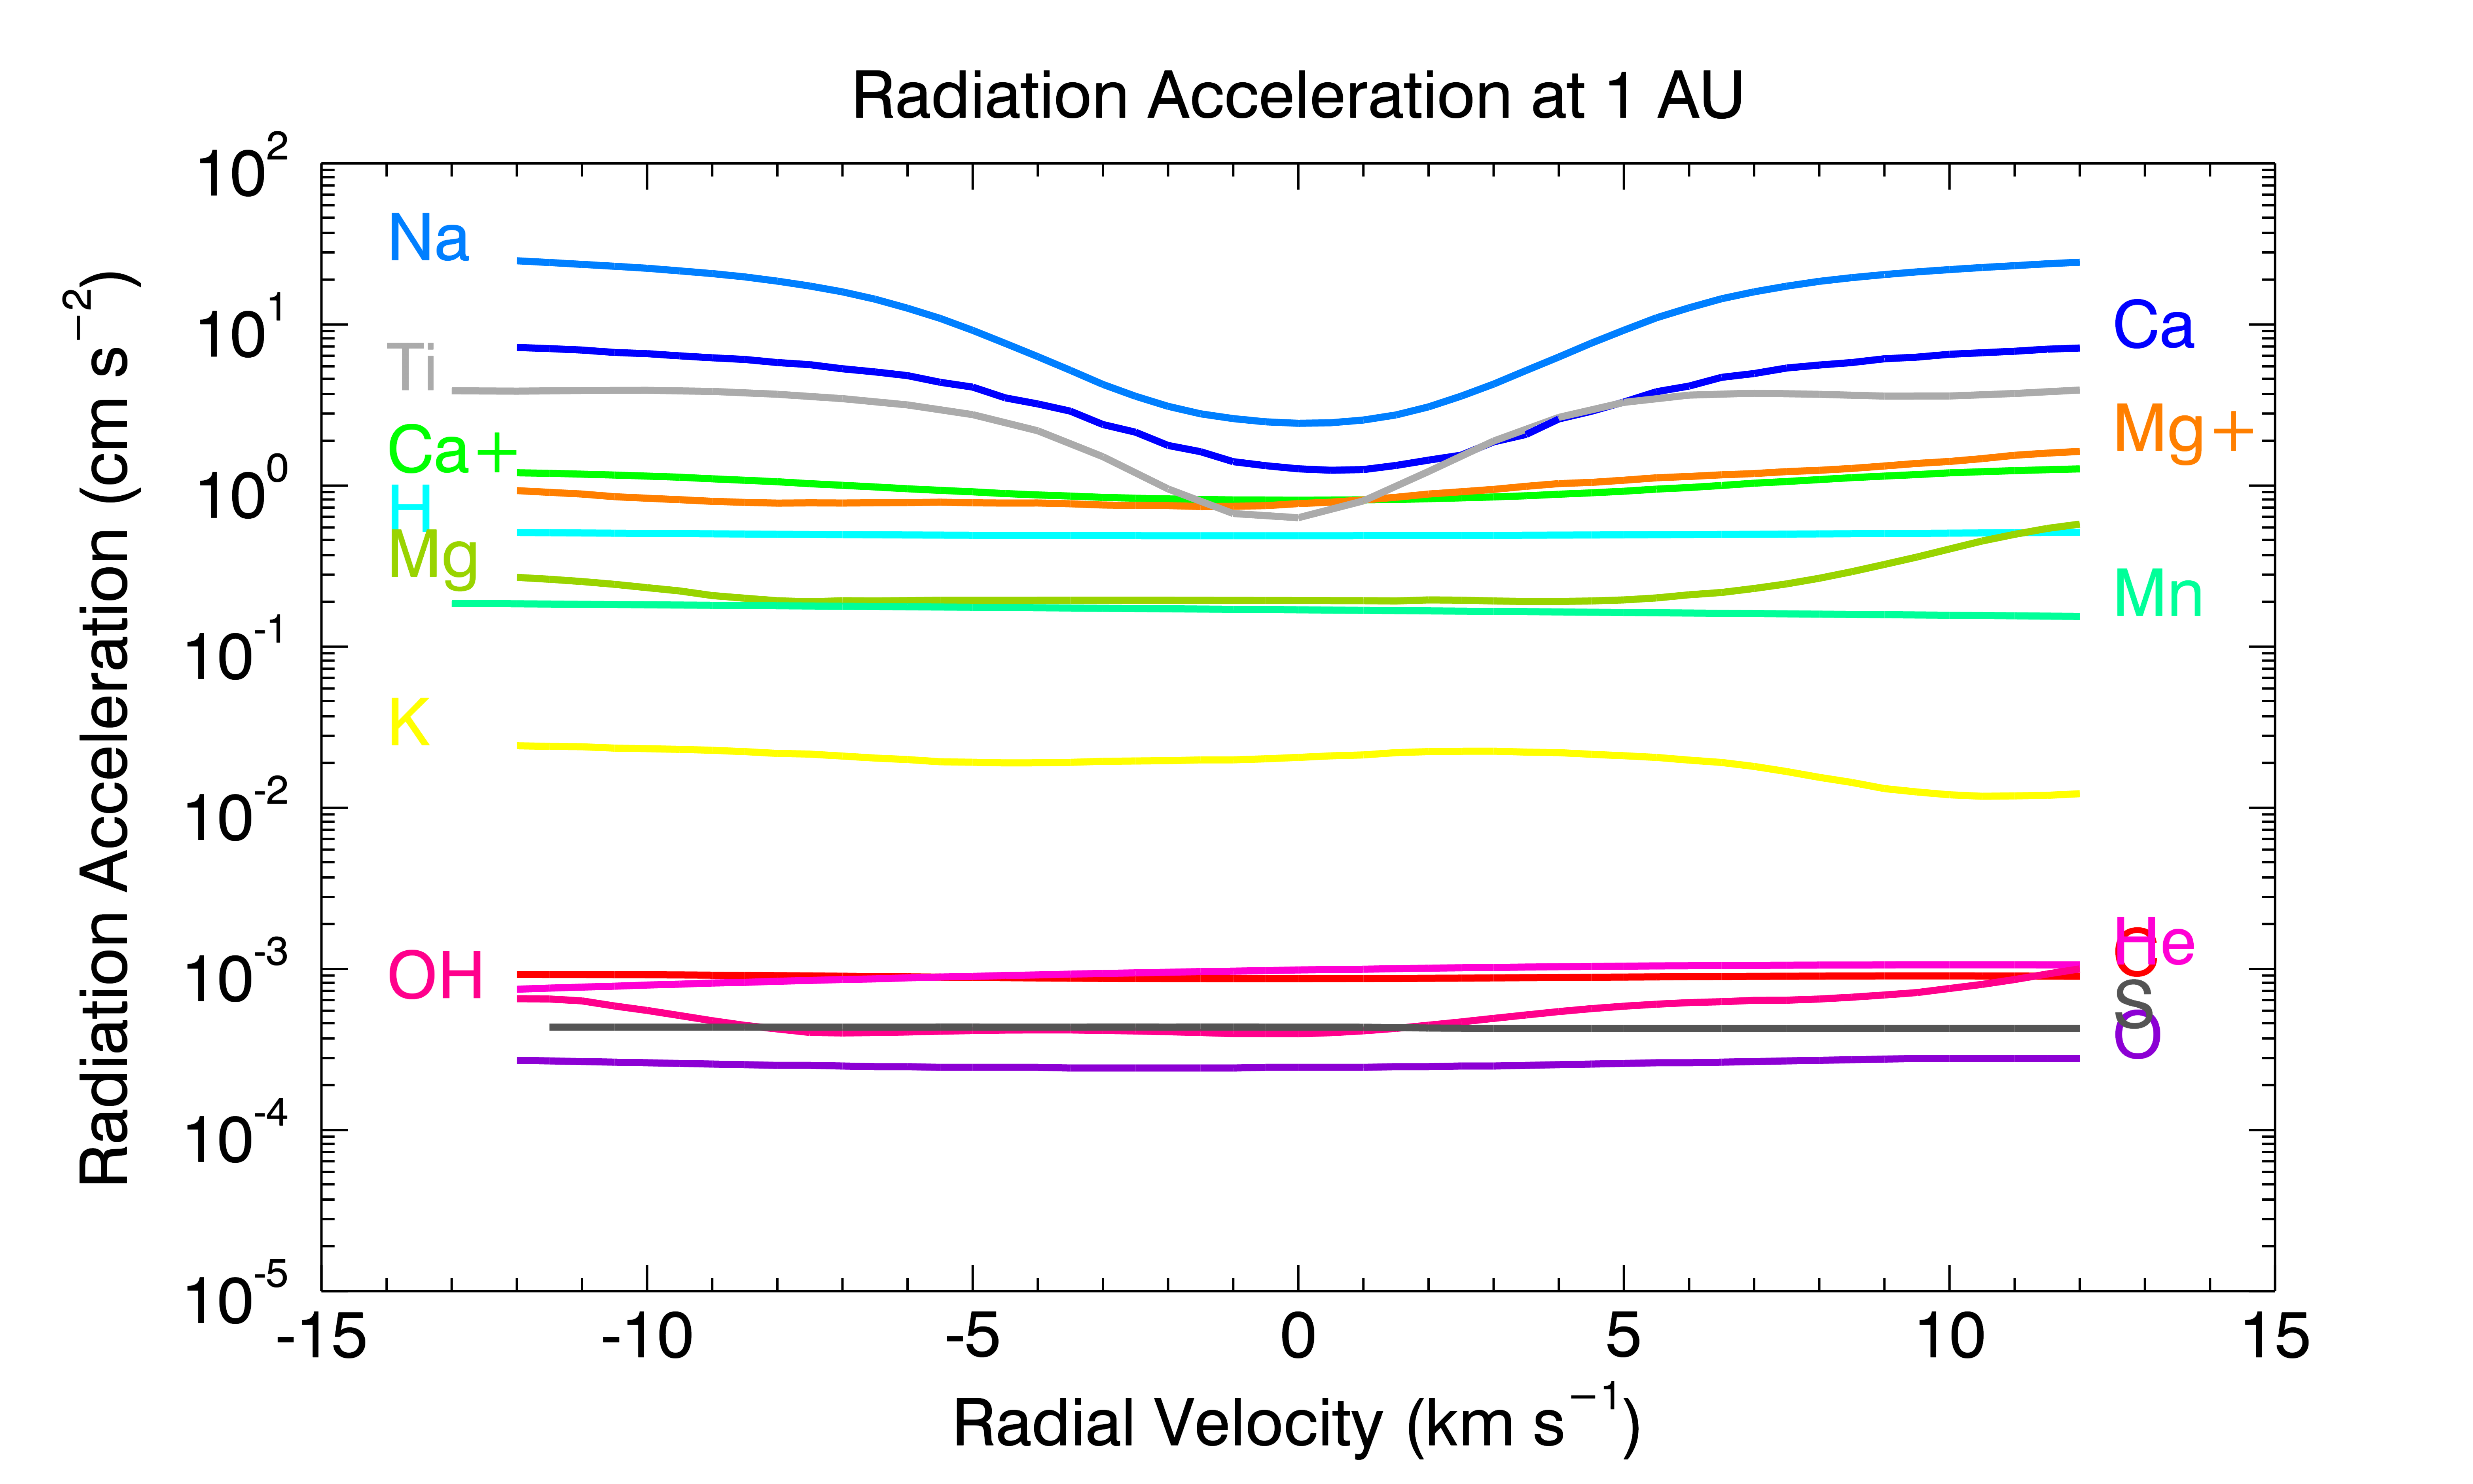
\includegraphics[width=\textwidth]{figures/radaccel.png}
\caption{Radiation acceleration as function of velocity for species with
available g-values.}
\label{fig:radaccel}
\end{figure}

\descrip{This Page Last Updated}
12 December 2011.

\clearpage
%%%%%%%%%%%%%%%%%%%%%%%%%%%%%%%%%%%%%%%%%%%%%%%%%%%%%%%%%%%%%%%%%%%%%%%%

\section{Integrator/driver\_3.2.pro} \label{sec:driver}

\descrip{Summary}

\descrip{Calling Procedure}

\descrip{Inputs}

\descrip{Outputs}

\descrip{Model Procedures Called}

\descrip{Notes}

\descrip{This Page Last Updated}

\clearpage
%%%%%%%%%%%%%%%%%%%%%%%%%%%%%%%%%%%%%%%%%%%%%%%%%%%%%%%%%%%%%%%%%%%%%%%%

\section{Integrator/rk5\_3.3.pro} \label{sec:rk5}

\descrip{Summary}
Computes a Runge-Kutta step and estimates the error.

\descrip{Calling Procedure}

\descrip{Inputs}

\descrip{Outputs}

\descrip{Model Procedures Called}

\descrip{Notes}
\begin{compactenum}
\item Based on Numerical Recipies, 3rd Edition, Ch.\ 17.2
\item The general form of a fifth-order Runge-Kutta formula is (NR, p.\ 912):
  \begin{eqnarray}
  k_1 & = & h f(x_n,y_n) \\
  k_2 & = & h f(x_n+c_2 h, y_n + a_{21} k_1) \\
  k_3 & = & h f(x_n+c_3 h, y_n + a_{31} k_1 + a_{32} k_2) \\
  k_4 & = & h f(x_n+c_4 h, y_n + a_{41} k_1 + a_{42} k_2 + a_{43} k_3) \\
  k_5 & = & h f(x_n+c_5 h, y_n + a_{51} k_1 + a_{52} k_2 + a_{53} k_3 + a_{54} k_4) \\
  k_6 & = & h f(x_n+c_6 h, y_n + a_{61} k_1 + a_{62} k_3 + a_{63} k_3 + a_{64} k_4 +
    a_{65} k_5) \\
  y_{n+1} & = & y_n + b_1 k_1 + b_2 k_2 + b_3 k_3 + b_4 k_4 + b_5 k_5 + b_6 k_6
  \end{eqnarray}
\item The coefficients are given in Table~\ref{table:rk_coefs}
\item $(x_n, y_n)$ are the values at the beginning of the interval. $(x_{n+1},y_{n+1})$
are the values at the end. Actually, there are 7 equations for each $y_n$ corresponding
to the 7 output values.
\item Solving this set of differential equations:
  \begin{eqnarray}
  \frac{dx}{dt} & = & v_x \\
  \frac{dy}{dt} & = & v_y \\
  \frac{dz}{dt} & = & v_z \\
  \frac{dv_x}{dt} & = & F_x(x,y,z,v_x,v_y,v_z) \\
  \frac{dv_y}{dt} & = & F_y(x,y,z,v_x,v_y,v_z) \\
  \frac{dv_z}{dt} & = & F_z(x,y,z,v_x,v_y,v_z) \\
  f & = & f_0 e^{-\nu(x,y,z,v_x,v_y,v_z) t}
  \end{eqnarray}
  
\begin{table}
\caption{5th Order Runge-Kutta Coefficeints}
\label{table:rk_coefs}
\end{table}

\end{compactenum}

\descrip{This Page Last Updated}
1 August 2012

\clearpage
%%%%%%%%%%%%%%%%%%%%%%%%%%%%%%%%%%%%%%%%%%%%%%%%%%%%%%%%%%%%%%%%%%%%%%%%

\section{Lifetimes/JupiterPlasma\_3.1.pro} \label{sec:JupiterPlasma}

\descrip{Summary}

\descrip{Calling Procedure}

\descrip{Inputs}

\descrip{Outputs}

\descrip{Model Procedures Called}

\descrip{Notes}

\descrip{This Page Last Updated}

\clearpage
%%%%%%%%%%%%%%%%%%%%%%%%%%%%%%%%%%%%%%%%%%%%%%%%%%%%%%%%%%%%%%%%%%%%%%%%

\section{Lifetimes/SaturnPlasma\_2.0.pro} \label{sec:SaturnPlasma}

\descrip{Summary}

\descrip{Calling Procedure}

\descrip{Inputs}

\descrip{Outputs}

\descrip{Model Procedures Called}

\descrip{Notes}

\descrip{This Page Last Updated}

\clearpage
%%%%%%%%%%%%%%%%%%%%%%%%%%%%%%%%%%%%%%%%%%%%%%%%%%%%%%%%%%%%%%%%%%%%%%%%

\section{Lifetimes/ionization\_rate\_3.3.pro} \label{sec:ionization_rate}

\descrip{Summary}

\descrip{Calling Procedure}

\descrip{Inputs}

\descrip{Outputs}

\descrip{Model Procedures Called}

\descrip{Notes}

\descrip{This Page Last Updated}

\clearpage
%%%%%%%%%%%%%%%%%%%%%%%%%%%%%%%%%%%%%%%%%%%%%%%%%%%%%%%%%%%%%%%%%%%%%%%%

\section{Lifetimes/lifetime\_setup\_3.2.pro} \label{sec:lifetime_setup}

\descrip{Summary}

\descrip{Calling Procedure}

\descrip{Inputs}

\descrip{Outputs}

\descrip{Model Procedures Called}

\descrip{Notes}

\descrip{This Page Last Updated}

\clearpage
%%%%%%%%%%%%%%%%%%%%%%%%%%%%%%%%%%%%%%%%%%%%%%%%%%%%%%%%%%%%%%%%%%%%%%%%

\section{Lifetimes/load\_plasma\_2.1.pro} \label{sec:load_plasma}

\descrip{Summary}

\descrip{Calling Procedure}

\descrip{Inputs}

\descrip{Outputs}

\descrip{Model Procedures Called}

\descrip{Notes}

\descrip{This Page Last Updated}

\clearpage
%%%%%%%%%%%%%%%%%%%%%%%%%%%%%%%%%%%%%%%%%%%%%%%%%%%%%%%%%%%%%%%%%%%%%%%%

\section{Lifetimes/xyz\_to\_magcoord\_3.1.pro} \label{sec:xyz_to_magcood}

\descrip{Summary}

\descrip{Calling Procedure}

\descrip{Inputs}

\descrip{Outputs}

\descrip{Model Procedures Called}

\descrip{Notes}

\descrip{This Page Last Updated}

\clearpage
%%%%%%%%%%%%%%%%%%%%%%%%%%%%%%%%%%%%%%%%%%%%%%%%%%%%%%%%%%%%%%%%%%%%%%%%

\section{ModelIO/BennaPrecipitationFilename\_1.0.pro}
\label{sec:BennaPrecipitationFilename}

\descrip{Summary}

\descrip{Calling Procedure}

\descrip{Inputs}

\descrip{Outputs}

\descrip{Model Procedures Called}

\descrip{Notes}

\descrip{This Page Last Updated}

\clearpage
%%%%%%%%%%%%%%%%%%%%%%%%%%%%%%%%%%%%%%%%%%%%%%%%%%%%%%%%%%%%%%%%%%%%%%%%

\section{$\checkmark$ModelIO/MercuryModelEndTime\_1.0.pro} \label{sec:MercuryModelEndTime}

\descrip{Summary}
Computes the appropriate value of \textit{input.options.endtime} for a Mercury
model run as a function of true anomaly angle. The appropriate value is set at
$4\times$ the photoionization lifetime.

\descrip{Calling Procedure}
\verb+endtime = MercuryModelEndTime(atoms, taa)+

\descrip{Inputs}
\begin{compactenum} \listup
\item atoms = species to look at
\item taa = true anomaly angle in radians
\end{compactenum}

\descrip{Outputs}
Function returns $4\times$ the photoionization lifetime of each species at the
requested true anomaly angles.

\descrip{Model Procedures Called}
\begin{compactenum} \listup
\item \hyperref[sec:planet_dist]{planet\_dist}: determines Mercury's distance
from the sun as function of true anomaly.
\item search\_atomicdata [not in the manual yet]
\end{compactenum}

\descrip{Notes}
None.

\descrip{This Page Last Updated}
12 December 2011

\clearpage
%%%%%%%%%%%%%%%%%%%%%%%%%%%%%%%%%%%%%%%%%%%%%%%%%%%%%%%%%%%%%%%%%%%%%%%%

\section{ModelIO/combine\_iterations\_3.2.pro} \label{sec:combine_iterations}

\descrip{Summary}

\descrip{Calling Procedure}

\descrip{Inputs}

\descrip{Outputs}

\descrip{Model Procedures Called}

\descrip{Notes}

\descrip{This Page Last Updated}

\clearpage
%%%%%%%%%%%%%%%%%%%%%%%%%%%%%%%%%%%%%%%%%%%%%%%%%%%%%%%%%%%%%%%%%%%%%%%%

\section{ModelIO/compare\_inputs\_3.0.pro} \label{sec:compare_inputs}

\descrip{Summary}

\descrip{Calling Procedure}

\descrip{Inputs}

\descrip{Outputs}

\descrip{Model Procedures Called}

\descrip{Notes}

\descrip{This Page Last Updated}

\clearpage
%%%%%%%%%%%%%%%%%%%%%%%%%%%%%%%%%%%%%%%%%%%%%%%%%%%%%%%%%%%%%%%%%%%%%%%%

\section{ModelIO/extract\_distribution\_3.3.pro}
\label{sec:extract_distribution}

\descrip{Summary}

\descrip{Calling Procedure}

\descrip{Inputs}

\descrip{Outputs}

\descrip{Model Procedures Called}

\descrip{Notes}

\descrip{This Page Last Updated}

\clearpage
%%%%%%%%%%%%%%%%%%%%%%%%%%%%%%%%%%%%%%%%%%%%%%%%%%%%%%%%%%%%%%%%%%%%%%%%

\section{ModelIO/extract\_parameter\_3.0.pro} \label{sec:extract_parameter}

\descrip{Summary}

\descrip{Calling Procedure}

\descrip{Inputs}

\descrip{Outputs}

\descrip{Model Procedures Called}

\descrip{Notes}

\descrip{This Page Last Updated}

\clearpage
%%%%%%%%%%%%%%%%%%%%%%%%%%%%%%%%%%%%%%%%%%%%%%%%%%%%%%%%%%%%%%%%%%%%%%%%

\section{ModelIO/inputs\_restore\_3.3.pro} \label{sec:inputs_restore}

\descrip{Summary}

\descrip{Calling Procedure}

\descrip{Inputs}

\descrip{Outputs}

\descrip{Model Procedures Called}

\descrip{Notes}

\descrip{This Page Last Updated}

\clearpage
%%%%%%%%%%%%%%%%%%%%%%%%%%%%%%%%%%%%%%%%%%%%%%%%%%%%%%%%%%%%%%%%%%%%%%%%

\section{ModelIO/make\_generic\_input\_3.1.pro} \label{sec:make_generic_input}

\descrip{Summary}

\descrip{Calling Procedure}

\descrip{Inputs}

\descrip{Outputs}

\descrip{Model Procedures Called}

\descrip{Notes}

\descrip{This Page Last Updated}

\clearpage
%%%%%%%%%%%%%%%%%%%%%%%%%%%%%%%%%%%%%%%%%%%%%%%%%%%%%%%%%%%%%%%%%%%%%%%%

\section{ModelIO/make\_model\_header\_3.2.pro} \label{sec:make_model_header}

\descrip{Summary}

\descrip{Calling Procedure}

\descrip{Inputs}

\descrip{Outputs}

\descrip{Model Procedures Called}

\descrip{Notes}

\descrip{This Page Last Updated}

\clearpage
%%%%%%%%%%%%%%%%%%%%%%%%%%%%%%%%%%%%%%%%%%%%%%%%%%%%%%%%%%%%%%%%%%%%%%%%

\section{ModelIO/modeloutput\_search\_3.5.pro} \label{sec:modeloutput_search}

\descrip{Summary}

\descrip{Calling Procedure}

\descrip{Inputs}

\descrip{Outputs}

\descrip{Model Procedures Called}

\descrip{Notes}

\descrip{This Page Last Updated}

\clearpage
%%%%%%%%%%%%%%%%%%%%%%%%%%%%%%%%%%%%%%%%%%%%%%%%%%%%%%%%%%%%%%%%%%%%%%%%

\section{ModelIO/output\_filename\_3.5.pro} \label{sec:output_filename}

\descrip{Summary}

\descrip{Calling Procedure}

\descrip{Inputs}

\descrip{Outputs}

\descrip{Model Procedures Called}

\descrip{Notes}

\descrip{This Page Last Updated}

\clearpage
%%%%%%%%%%%%%%%%%%%%%%%%%%%%%%%%%%%%%%%%%%%%%%%%%%%%%%%%%%%%%%%%%%%%%%%%

\section{$\checkmark$ModelIO/print\_inputs\_3.1.pro} \label{sec:print_inputs}

\descrip{Summary}
Prints the contents of an input structure to the screen.

\descrip{Calling Procedure}
\verb+print_inputs, input, printarr=printarr+

\descrip{Inputs}
\begin{compactenum} \listup
\item input: either an input structure or the name on an inputfile
\end{compactenum}

\descrip{Outputs}
\begin{compactenum} \listup
\item printarr: contains a strarr with each of the input fields
\end{compactenum}

\descrip{Model Procedures Called}
\begin{compactenum} \listup
\item \hyperref[sec:inputs_restore]{inputs\_restore}
\end{compactenum}

\descrip{Notes}
None.

\descrip{This Page Last Updated}
9 December 2011.

\clearpage
%%%%%%%%%%%%%%%%%%%%%%%%%%%%%%%%%%%%%%%%%%%%%%%%%%%%%%%%%%%%%%%%%%%%%%%%

\section{SourceDistributions/PSD\_distribution\_1.1.pro}
\label{sec:PSD_distribution}

\descrip{Summary}

\descrip{Calling Procedure}

\descrip{Inputs}

\descrip{Outputs}

\descrip{Model Procedures Called}

\descrip{Notes}

\descrip{This Page Last Updated}

\clearpage
%%%%%%%%%%%%%%%%%%%%%%%%%%%%%%%%%%%%%%%%%%%%%%%%%%%%%%%%%%%%%%%%%%%%%%%%

\section{SourceDistributions/SO2exosphere\_distribution\_3.2.pro}
\label{sec:SO2exosphere_distribution}

\descrip{Summary}

\descrip{Calling Procedure}

\descrip{Inputs}

\descrip{Outputs}

\descrip{Model Procedures Called}

\descrip{Notes}

\descrip{This Page Last Updated}

\clearpage
%%%%%%%%%%%%%%%%%%%%%%%%%%%%%%%%%%%%%%%%%%%%%%%%%%%%%%%%%%%%%%%%%%%%%%%%

\section{SourceDistributions/SourceFlux\_1.0.pro} \label{sec:sourceflux}

\descrip{Summary}

\descrip{Calling Procedure}

\descrip{Inputs}

\descrip{Outputs}

\descrip{Model Procedures Called}

\descrip{Notes}

\descrip{This Page Last Updated}

\clearpage
%%%%%%%%%%%%%%%%%%%%%%%%%%%%%%%%%%%%%%%%%%%%%%%%%%%%%%%%%%%%%%%%%%%%%%%%

\section{SourceDistributions/SourceRate\_1.0.pro} \label{sec:sourcerate}

\descrip{Summary}

\descrip{Calling Procedure}

\descrip{Inputs}

\descrip{Outputs}

\descrip{Model Procedures Called}

\descrip{Notes}

\descrip{This Page Last Updated}

\clearpage
%%%%%%%%%%%%%%%%%%%%%%%%%%%%%%%%%%%%%%%%%%%%%%%%%%%%%%%%%%%%%%%%%%%%%%%%

\section{SourceDistributions/add\_perturbation\_2.2.pro}
\label{sec:addperturbation}

\descrip{Summary}

\descrip{Calling Procedure}

\descrip{Inputs}

\descrip{Outputs}

\descrip{Model Procedures Called}

\descrip{Notes}

\descrip{This Page Last Updated}

\clearpage
%%%%%%%%%%%%%%%%%%%%%%%%%%%%%%%%%%%%%%%%%%%%%%%%%%%%%%%%%%%%%%%%%%%%%%%%

\section{SourceDistributions/angular\_distribution\_3.1.pro}
\label{sec:angulardistribution}

\descrip{Summary}
Determines the initial angular distribution for packets.

\descrip{Calling Procedure}
\verb+angular_distribution, input, output, npack, seed+

\descrip{Inputs}
\begin{compactenum} \listup
\item input = input structure
\item output = output structure with \textit{output.vx0}=initial speed distribution.
\item npack = number of packets
\item seed = seed for random number generator
\end{compactenum} 

\descrip{Outputs}
\begin{compactenum} \listup
\item output = output structure with \textit{output.vx0}, \textit{output.vy0}, and
\textit{output.vz0} defined in units of \Rplan\ s$^{-1}$
\end{compactenum} 

\descrip{Model Procedures Called}
\begin{compactenum} \listup
\item \texttt{random\_nr}
\item \texttt{RandomDeviates\_1d}
\end{compactenum}

\descrip{Notes}
\begin{compactenum} \listup
\item First step: randomly choose altitude ($\theta$) and azimuth ($\phi$) angles.
  \begin{compactenum}
  \item Altitude is measured from surface tangent ($\theta=0$) to surface normal
  ($\theta=\pi/2$).
  \item The zero point for azimuth angle is not clear to me. It is possible to limit the
  azimuth angle, but I'm not sure exactly how the zero point is defined at each point on
  the surface. It is better to use the default ($0 \leq \phi \leq 2\pi$.
  \item Three options for \textit{angulardist.type}: \texttt{radial}, \texttt{isotropic},
    \texttt{costheta}
  \item Radial ejection
    \begin{compactenum}
    \item $\theta = \pi/2$ for all packets
    \item $\phi = 0$ for all packets (azimuth angle is technically undefined for normal
    ejection.
    \end{compactenum}
  \item Isotropic ejection
    \begin{compactenum} 
    \item Azimuth angles are evenly distributed from $0 \rightarrow 2\pi$.
    \item $\sin \theta$ is evenly distributed between $0 \rightarrow 1$ for distributions
    that start at the surface ($2\pi$ ejection into outward-facing hemisphere) or 
    $-1 \rightarrow 1$ for ejection into $4\pi$ str.
    \end{compactenum}
  \item costheta ejection
    \begin{compactenum}
    \item Azimuth angles are evenly distributed from $0 \rightarrow 2\pi$.
    \item $f(\sin \theta) = \sin^n \theta$
    \end{compactenum}
  \end{compactenum}
\end{compactenum}

\descrip{This Page Last Updated}
20 January 2012

\clearpage
%%%%%%%%%%%%%%%%%%%%%%%%%%%%%%%%%%%%%%%%%%%%%%%%%%%%%%%%%%%%%%%%%%%%%%%%

\section{SourceDistributions/charge\_exchange\_perturbation\_2.0.pro}
\label{sec:charge_exchange_perturbation}

\descrip{Summary}

\descrip{Calling Procedure}

\descrip{Inputs}

\descrip{Outputs}

\descrip{Model Procedures Called}

\descrip{Notes}

\descrip{This Page Last Updated}

\clearpage
%%%%%%%%%%%%%%%%%%%%%%%%%%%%%%%%%%%%%%%%%%%%%%%%%%%%%%%%%%%%%%%%%%%%%%%%

\section{SourceDistributions/exosphere\_distribution\_3.0.pro}
\label{sec:exosphere_distribution}

\descrip{Summary}

\descrip{Calling Procedure}

\descrip{Inputs}

\descrip{Outputs}

\descrip{Model Procedures Called}

\descrip{Notes}

\descrip{This Page Last Updated}

\clearpage
%%%%%%%%%%%%%%%%%%%%%%%%%%%%%%%%%%%%%%%%%%%%%%%%%%%%%%%%%%%%%%%%%%%%%%%%

\section{SourceDistributions/show\_veldist\_1.0.pro} \label{sec:show_veldist}

\descrip{Summary}

\descrip{Calling Procedure}

\descrip{Inputs}

\descrip{Outputs}

\descrip{Model Procedures Called}

\descrip{Notes}

\descrip{This Page Last Updated}

\clearpage
%%%%%%%%%%%%%%%%%%%%%%%%%%%%%%%%%%%%%%%%%%%%%%%%%%%%%%%%%%%%%%%%%%%%%%%%

\section{$\checkmark$SourceDistributions/source\_distribution\_3.3.pro}
\label{sec:source_distribution}

\descrip{Summary}
Determines the initial positions and velocities for each packet. This is a
driver program which calls the procuedures to determine initial spatial, speed,
and angular distributions of packets.

\descrip{Calling Procedure}
\verb+source_distribution, input, npack, seed, output=output+

\descrip{Inputs}
\begin{compactenum} \listup
\item input: \texttt{input} structure
\item npack: number of packets in the output
\item seed: seed for random number generator (optional)
\end{compactenum}

\descrip{Outputs}
\begin{compactenum} \listup
\item output: an \texttt{output} structure (see below)
\end{compactenum}

\descrip{Model Procedures Called}
\begin{compactenum} \listup
\item random\_nr
\item \hyperref[sec:surface_distribution]{surface\_distribution}
\item \hyperref[sec:torus_distribution]{torus\_distribution}
\item \hyperref[sec:exosphere_distribution]{exosphere\_distribution}
\item \hyperref[sec:SO2exosphere_distribution]{SO2exosphere\_distribution}
\item \hyperref[sec:PSD_distribution]{PSD\_distribution}
\item \hyperref[sec:speed_distribution]{speed\_distribution}
\item \hyperref[sec:angular_distribution]{angular\_distribution}
\item \hyperref[sec:add_perturbation]{add\_perturbation}
\item \hyperref[sec:locmoon]{locmoon}
\end{compactenum}

\descrip{Notes}
Procuedure used:
\begin{compactenum} 
\item Create the \texttt{output} structure (see
Table~\ref{table:outputstructure} for description of fields). This just sets up
the structure put does not put any values into the fields.

\item \texttt{output.f0} = 1 for all packets initially.

\item Set the output time: \\
  \begin{compactitem} \vspace{-\baselineskip}
  \item If \texttt{input.options.at\_once = }1, then
  \texttt{output.time} is set to \texttt{input.options.endtime} for all
  packets. 
  \item If \texttt{input.options.at\_once = 0}, then \texttt{output.time} is
  set to a random value between 0 and \texttt{input.options.endtime}.
  \end{compactitem}

\item Set the initial locations for packets. Possible distributions allowed in
\texttt{input.SpatailDist.type} are:
  \begin{compactitem} 
  \item \textit{surface}: starts all packets at a sphere located at
    \texttt{input.geometry.startpoint}'s surface or a uniform exobase. See
    \hyperref[sece:surface_distribution]{surface\_distribution}
  \item \textit{torus}: starts all packets in a uniform torus around
    \texttt{input.geometry.startpoint}. 
    See \hyperref[sec:torus_distribution]{torus\_distribution}
  \item \textit{exosphere}: starts all the packets in an exosphere over the
    surface of \texttt{input.geometry.startpoint}
    See \hyperref[sec:exosphere_distribution]{exosphere\_distribution}
  \item \textit{SO2 exosphere}: Uses Vincent Dol's exospheric source model.
    See \hyperref[sec:SO2exosphere_distribution]{SO2exosphere\_distribution}
  \item \textit{PSD distribution}: Approximation to the ion-enhanced PSD
  distribution described by \citet{burger2010}. See 
  \hyperref[sec:PSD_distribution]{PSD\_distribution}
  \end{compactitem}
These routines set \texttt{output.x0}, \texttt{output.y0}, and
\texttt{output.z0} in a coordinate system centered on
\texttt{input.geometry.startpoint}. A transformation to the
\texttt{input.geometry.planet}-cenetered coordinate system is made later, if
necessary.

\item Set the initial speed distribution. See
\hyperref[sec:speed_distribution]{speed\_distribution}. This routine sets the
intitial speed (and possibly the components of the speed) in units of \Rplan\
s$^{-1}$. Satellite orbital velocity is not included yet.

\item Set the angular disitribution, if necessary. See
\hyperref[sec:angular_distribution]{angular\_distribution}. This routine sets
\texttt{output.vx0}, \texttt{output.vy0}, and \texttt{output.vz0} (if it has not
already been done) in a coordinate system centered on
\texttt{input.geometry.startpoint}. A transformation to the
\texttt{input.geometry.planet}-cenetered coordinate system is made later, if
necessary.

\item Add a perturbation to the intial velocities, if requested. See 
\hyperref[sec:add_perturbation]{add\_perturbation}.

\item Make the conversion from the \texttt{input.geometry.startpoint}-centered
system to the \texttt{input.geometry.planet}-cenetered system if necessary.
  \begin{compactenum}
  \item Move the packets out to their starting distance and rescale from
  $\mathrm{R_{st.pt.}}$ to \Rplan:
    \begin{eqnarray}
    x & = & x_0 \times \text{\texttt{SystemConsts.radius}} \\
    y & = & y_0 \times \text{\texttt{SystemConsts.radius}} +
      \text{\texttt{SystemConsts.a}} \\
    z & = & z_0 \times \text{\texttt{SystemConsts.radius}}
    \end{eqnarray}
   This places each packet at the satellite's orbital distance at orbital phase
   = 0\degr\ (local midnight).
  \item Add in the orbital velocity, if \texttt{input.options.motion=1}:
    \begin{eqnarray}
    v_x & = & vx_0 \\
    v_y & = & vy_0 - \text{\texttt{SystemConsts.orbvel}} \\
    v_z & = & vz_0
    \end{eqnarray}
    For a packet at orbital phase = 0\degr, the direction of orbital motion is
    in the $-\hat{y}$ direction.
  \item Determine \texttt{output.phi0}, the orbital phase of the satellite at
  the start time of each packet 
  (\texttt{output.time} seconds ago). See \hyperref[sec:locmoon]{locmoon}.

  \item Rotate the packets to the proper location in planet-centered
  coordinates:
    \begin{eqnarray}
    output.x & = & x \cos \phi_0 - y \sin \phi_0 \\
    output.y & = & x \sin \phi_0 + y \cos \phi_0 \\
    output.z & = & z \\ 
    output.vx & = & v_x \cos \phi_0 - v_y \sin \phi_0 \\
    output.vy & = & v_x \sin \phi_0 + v_y \cos \phi_0 \\
    output.vz & = & v_z 
    \end{eqnarray}
  \end{compactenum}
  
\item \texttt{output.x0}, etc., are in startpoint-centered coordinates. These
are not used in any of the model computations.
\item \texttt{output.x}, etc., are in planet-centered coordinates. These are
used in all of the model computations.
\end{compactenum}


\descrip{This Page Last Updated}
20 December 2011.

\clearpage
%%%%%%%%%%%%%%%%%%%%%%%%%%%%%%%%%%%%%%%%%%%%%%%%%%%%%%%%%%%%%%%%%%%%%%%%

\section{SourceDistributions/speed\_distribution\_3.3.pro}
\label{sec:speed_distribution}

\descrip{Summary}

\descrip{Calling Procedure}

\descrip{Inputs}

\descrip{Outputs}

\descrip{Model Procedures Called}

\descrip{Notes}

\descrip{This Page Last Updated}

\clearpage
%%%%%%%%%%%%%%%%%%%%%%%%%%%%%%%%%%%%%%%%%%%%%%%%%%%%%%%%%%%%%%%%%%%%%%%%

\section{SourceDistributions/speed\_dists\_2.1.pro} \label{sec:speed_dists}

\descrip{Summary}

\descrip{Calling Procedure}

\descrip{Inputs}

\descrip{Outputs}

\descrip{Model Procedures Called}

\descrip{Notes}

\descrip{This Page Last Updated}

\clearpage
%%%%%%%%%%%%%%%%%%%%%%%%%%%%%%%%%%%%%%%%%%%%%%%%%%%%%%%%%%%%%%%%%%%%%%%%

\section{SourceDistributions/surface\_distribution\_3.2.pro}
\label{sec:surface_distribution}

\descrip{Summary}
Distribute packets about a sphere with radius r = 
  \texttt{input.SpatialDist.exobase}

\descrip{Calling Procedure}
\verb+surface_distribution, input, output, npack, seed+

\descrip{Inputs}
\begin{compactenum} \listup
\item input: \texttt{input} structure
\item output: \texttt{output} structure defined in
\hyperref[sec:source_distribution]{source\_distribution}
(Table~\ref{table:outputstructure})
\item npack: number of packets in the output
\item seed: seed for random number generator (optional)
\end{compactenum}

\descrip{Outputs}
\begin{compactenum} \listup
\item output: \texttt{output.x0}, \texttt{output.y0}, and \texttt{output.z0}
fields are populated.
\end{compactenum}

\descrip{Model Procedures Called}
\begin{compactenum} \listup
\item RandomDeviates\_2d
\item random\_nr
\end{compactenum}

\descrip{Notes}
There are several ways to use this option:
\begin{compactenum}
\item Use a predefined map file:
  \begin{compactenum}
  \item The following lines must be included in the \textit{input} file.
\begin{verbatim} 
SpatialDist.type = surface
SpatialDist.use_map = 1
SpatialDist.mapfile = path_to_mapfile
\end{verbatim}
  \item \textit{mapfile} is an IDL savefile with a variable called
  \texttt{sourcemap} which is a structure defined by: 
\begin{verbatim}
sourcemap = {longitude:ptr_new(longitude), latitude:ptr_new(latitude), $
  map:ptr_new(map)} 
\end{verbatim}
  where:
    \begin{compactitem}
    \item \texttt{longitude} is an array of longitude ($\lambda$) values in 
    radians. See
    Section~\ref{sec:coordsystems} for definition of longitude. The acceptable
    range of values is $0 \leq \lambda \leq 2\pi$. I generally set
    this to: \\ \verb+longitude = fltarr(361)*!dtor}+
    \item \texttt{latitude} is an array of latitude ($\mu$) values in radians. 
    The acceptable range of values is $-\pi/2 \leq \mu \leq \pi/2$. I
    generally set this to \\ \verb+latitude = fltarr(181)*!dtor - !pi/2.+
    \item \texttt{map} is an array of size ($n_\lambda,n_\mu$) containing the
    relative source flux (particles per unit area) as a function of $\lambda$
    and $\mu$. This does not need to be absolute flux since it is normalized to
    the total number of packets ejected.
    \end{compactitem}
  \end{compactenum}
\item Uniform ejection within a specified range
  \begin{compactenum}
  \item The following lines must be included in the input file:
  \begin{verbatim}
SpatialDist.type = surface
SpatialDist.use_map = 0
  \end{verbatim}
  The following lines are optional:
  \begin{verbatim}
SpatialDist.longitude0 = minlong
SpatialDist.longitude1 = maxlong
SpatialDist.latitude0 = minlat
SpatialDist.latitude1 = maxlat
  \end{verbatim}
  \item \texttt{minlong} ($\lambda_{min}$) and \texttt{maxlong}
  ($\lambda_{max}$) are the minimum and maximum longitude values with 
  $0 \leq \lambda_{min},\lambda_{max} \leq 2\pi$.
    \begin{compactitem}
    \item If $\lambda_{min} < \lambda_{max}$, then packets are randomly
    distributed with $\lambda_{min} \leq \lambda < \lambda_{max}$
    (Figure~\ref{fig:surfdist0}a).
    \item If $\lambda_{min} > \lambda_{max}$, then packets are randomly
    distributed with $\lambda_{max} \leq \lambda < \lambda_{max}+2\pi$
    (Figure~\ref{fig:surfdist0}b).
    \item If $\lambda_{min} = \lambda_{max}$ then all packets are set to
    $\lambda = \lambda_{min}$.
    \end{compactitem}
  \item \texttt{minlat} ($\mu_{min}$) and \texttt{maxlat} ($\mu_{max}$) are the
  minimum and maximum values of latitude with $\pi/2 \leq \mu_{min} \leq 
  \mu_{max} \leq \pi/2$.
  \item Default values:
    \begin{eqnarray*}
    \lambda_{min} & = & 0 \\
    \lambda_{max} & = & 2\pi \\
    \mu_{min} & = & -\pi/2 \\
    \mu_{max} & = & \pi/2 
    \end{eqnarray*}
  \end{compactenum}
\item Choosing random values:
  \begin{compactenum}
  \item Longitude values are evenly distributed between $\lambda_{min}$ and
  $\lambda_{max}$, so we can choose values with: 
    \begin{equation}
    \lambda = \lambda_{min} + (\lambda_{max}-\lambda_{min}) R
    \end{equation}
    where $R$ is a random deviate from a uniform distribution with $0 \leq R <
    1$.
  \item Latitude values are not evenly distributed; however, $\sin \mu$ are, so
  we can choose values with:
    \begin{equation}
    \sin \mu = \sin \mu_{min} + (\sin \mu_{max}-\sin \mu_{min}) R 
    \end{equation}
    where $R$ is a random number as above and $-1 \leq \sin \mu < 1$.
  \end{compactenum}
\item If \texttt{input.geometry.StartPoint = input.geometry.planet} then:
  \begin{compactitem}
  \item local noon: $\lambda=0$\degr, $(x,y,z)=(0,-1,0)$
  \item local dusk: $\lambda=90$\degr, $(x,y,z)=(1,0,0)$
  \item local midnight: $\lambda=180$\degr, $(x,y,z)=(0,1,0)$
  \item local dawn: $\lambda=270$\degr, $(x,y,z)=(-1,0,0)$
  \end{compactitem}
  \begin{eqnarray}
  x_0 & = & r_0 \sin \lambda \cos \mu \\
  y_0 & = & -r_0 \cos \lambda \sin \mu \\
  z_0 & = & r_0 \sin \mu
  \end{eqnarray}
  where $r_0$ = \texttt{input.SpatialDist.exobase}
\item If \texttt{input.geometry.StartPoint $\neq$ input.geometry.planet}
then:  
  \begin{compactitem}
  \item sub-planet: $\lambda=0$\degr, $(x,y,z)=(0,-1,0)$
  \item leading side: $\lambda=90$\degr, $(x,y,z)=(1,0,0)$
  \item anti-planet: $\lambda=180$\degr, $(x,y,z)=(0,1,0)$
  \item trailing side: $\lambda=270$\degr, $(x,y,z)=(-1,0,0)$
  \end{compactitem}
  \begin{eqnarray}
  x_0 & = & -r_0 \sin \lambda \cos \mu \\
  y_0 & = & -r_0 \cos \lambda \cos \mu \\
  z_0 & = & r_0 \sin \mu
  \end{eqnarray}
\end{compactenum}

\descrip{This Page Last Updated}
21 December 2011.

\begin{figure}[h]
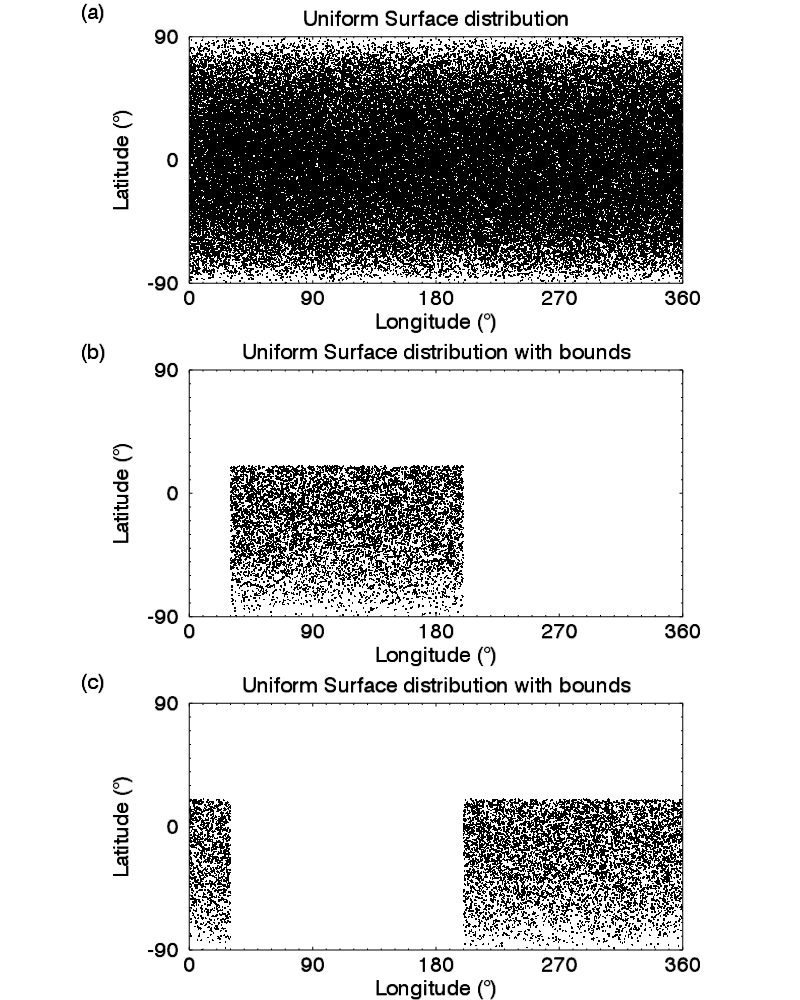
\includegraphics[width=\textwidth]{figures/surfdist0.png}
\caption{(a) $10^5$ packets randomly distributed in longitude and latitude over
a surface. 
(b) $10^4$ packets randomly distributed over a surface with
$\lambda_{min}=30^\circ$, $\lambda_{max}=200^{\circ}$, $\mu_{min}=-90^{\circ}$,
and $\mu_{max}=20^{\circ}$.
(c) $10^4$ packets randomly distributed over a surface with
$\lambda_{min}=200^\circ$, $\lambda_{max}=30^{\circ}$, $\mu_{min}=-90^{\circ}$,
and $\mu_{max}=20^{\circ}$.}
\label{fig:surfdist0}
\end{figure}

\clearpage
%%%%%%%%%%%%%%%%%%%%%%%%%%%%%%%%%%%%%%%%%%%%%%%%%%%%%%%%%%%%%%%%%%%%%%%%

\section{SourceDistributions/surface\_temperature\_3.0.pro}
\label{sec:surface_temperature}

\descrip{Summary}

\descrip{Calling Procedure}

\descrip{Inputs}

\descrip{Outputs}

\descrip{Model Procedures Called}

\descrip{Notes}

\descrip{This Page Last Updated}

\clearpage
%%%%%%%%%%%%%%%%%%%%%%%%%%%%%%%%%%%%%%%%%%%%%%%%%%%%%%%%%%%%%%%%%%%%%%%%

\section{SourceDistributions/torus\_distribution\_2.0.pro}
\label{sec:torus_distribution}

\descrip{Summary}

\descrip{Calling Procedure}

\descrip{Inputs}

\descrip{Outputs}

\descrip{Model Procedures Called}

\descrip{Notes}

\descrip{This Page Last Updated}

\clearpage
%%%%%%%%%%%%%%%%%%%%%%%%%%%%%%%%%%%%%%%%%%%%%%%%%%%%%%%%%%%%%%%%%%%%%%%%

\section{loc\_operations\_3.0.pro} \label{sec:loc_operations}

\descrip{Summary}

\descrip{Calling Procedure}

\descrip{Inputs}

\descrip{Outputs}

\descrip{Model Procedures Called}

\descrip{Notes}

\descrip{This Page Last Updated}

\clearpage
%%%%%%%%%%%%%%%%%%%%%%%%%%%%%%%%%%%%%%%%%%%%%%%%%%%%%%%%%%%%%%%%%%%%%%%%

\section{$\checkmark$locmoon\_1.0.pro} \label{sec:locmoon}

\descrip{Summary}
Calculates the coordinates of each moon given a ``final'' orbital longitude and
a time difference. Determines where a moon was \textit{time} seconds ago.

\descrip{Calling Procedure}
\verb+locmoon, time, theta0, radius, orbrate, x=x, y=y, z=z, ang=ang+

\descrip{Inputs}
\begin{compactitem} \listup
\item time: time before moon was at \textit{theta0} (seconds)
\item theta0: final orbital longitude of each moon (radians). Corresponds to
the position at \textit{time=0}.
\item radius: orbital radius of each moon (\Rplan)
\item orbrate: angular speed of each moon (radians/sec)
\end{compactitem}

\descrip{Outputs}
\begin{compactitem} \listup
\item x: x-position of each moon relative to the planet \textit{time} seconds 
it was before it was at \textit{theta0} (\Rplan)
\item y: y-position of each moon relative to the planet \textit{time} seconds 
it was before it was at \textit{theta0} (\Rplan)
\item z: z-position of each moon relative to the planet \textit{time} seconds 
it was before it was at \textit{theta0} (\Rplan)
\item ang: orbital longitude \textit{time} seconds ago (radians)
\end{compactitem}

\descrip{Model Procedures Called}
None.

\descrip{Notes}
\begin{compactitem} \listup
\item \textit{time} and \textit{theta0} are arrays of length npackets. radius
and orbrate are arrays with length nobj (number of objects in the system which
are included in the model run).
\item The outputs are arrays of size (npackets x nobj) which give the location
(in model coordinates) of each satellite as seen by each packet.
\item $z \equiv 0$ \rarrow\ I have assumed satellites orbit in the planetary
equatorial planes.
\item Equations used:
  \begin{eqnarray}
  \theta & = & -t R + \theta_0 \\
  x & = & -r \sin\theta \\
  y & = & r \cos\theta 
  \end{eqnarray}
  where $\theta$ is \textit{ang}, $t$ is \textit{time}, $R$ is \textit{orbrate} 
  $\theta_0$ is \textit{theta0}, and $r$ is \textit{radius}.
\end{compactitem}

\descrip{This Page Last Updated}
9 December 2011

\clearpage
%%%%%%%%%%%%%%%%%%%%%%%%%%%%%%%%%%%%%%%%%%%%%%%%%%%%%%%%%%%%%%%%%%%%%%%%

\section{$\checkmark$model\_common\_blocks\_3.0.pro} \label{sec:model_common_blocks}

\descrip{Summary}
Initializes the common blocks used in the model

\descrip{Calling Procedure}
\verb+model_common_blocks+

\descrip{Inputs}
None.

\descrip{Outputs}
None.

\descrip{Model Procedures Called}
None.

\descrip{Notes}
Three common blocks are defined:

\begin{compactenum} \vspace{-12pt}
\item constants
  \begin{compactitem} 
  \item SystemConsts: See Table~\ref{table:systemconsts}
  \item DipoleConsts: See Table~\ref{table:dipoleconsts}
  \item stuff: See \hyperref[sec:modeldriver]{modeldriver}
  \end{compactitem}
\item ratecoefs
  \begin{compactitem} 
  \item kappa: See \hyperref[sec:modeldriver]{modeldriver} 
  \end{compactitem}
\item plasma
  \begin{compactitem} 
  \item plasma: See \hyperref[sec:modeldriver]{modeldriver}  
  \item plasmahot: See \hyperref[sec:modeldriver]{modeldriver}  
  \end{compactitem}
\end{compactenum}

\descrip{This Page Last Updated}
9 December 2011

\clearpage
%%%%%%%%%%%%%%%%%%%%%%%%%%%%%%%%%%%%%%%%%%%%%%%%%%%%%%%%%%%%%%%%%%%%%%%%

\section{model\_findpackets\_4.0.pro} \label{sec:model_findpackets}

\descrip{Summary}

\descrip{Calling Procedure}

\descrip{Inputs}

\descrip{Outputs}

\descrip{Model Procedures Called}

\descrip{Notes}

\descrip{This Page Last Updated}

\clearpage
%%%%%%%%%%%%%%%%%%%%%%%%%%%%%%%%%%%%%%%%%%%%%%%%%%%%%%%%%%%%%%%%%%%%%%%%

\section{modeldriver\_3.9.pro} \label{sec:modeldriver}

\descrip{Summary}

\descrip{Calling Procedure}

\descrip{Inputs}

\descrip{Outputs}

\descrip{Model Procedures Called}

\descrip{Notes}

\descrip{This Page Last Updated}

\clearpage
%%%%%%%%%%%%%%%%%%%%%%%%%%%%%%%%%%%%%%%%%%%%%%%%%%%%%%%%%%%%%%%%%%%%%%%%

\section{modelstreamlinesB\_3.0.pro} \label{sec:modelstreamlinesB}

\descrip{Summary}

\descrip{Calling Procedure}

\descrip{Inputs}

\descrip{Outputs}

\descrip{Model Procedures Called}

\descrip{Notes}

\descrip{This Page Last Updated}

\clearpage
%%%%%%%%%%%%%%%%%%%%%%%%%%%%%%%%%%%%%%%%%%%%%%%%%%%%%%%%%%%%%%%%%%%%%%%%

\section{modelstreamlines\_3.0.pro} \label{sec:modelstreamlines}

\descrip{Summary}

\descrip{Calling Procedure}

\descrip{Inputs}

\descrip{Outputs}

\descrip{Model Procedures Called}

\descrip{Notes}

\descrip{This Page Last Updated}

\clearpage
%%%%%%%%%%%%%%%%%%%%%%%%%%%%%%%%%%%%%%%%%%%%%%%%%%%%%%%%%%%%%%%%%%%%%%%%

\section{modstreamA\_3.0.pro} \label{sec:modstreamA}

\descrip{Summary}

\descrip{Calling Procedure}

\descrip{Inputs}

\descrip{Outputs}

\descrip{Model Procedures Called}

\descrip{Notes}

\descrip{This Page Last Updated}

\clearpage
%%%%%%%%%%%%%%%%%%%%%%%%%%%%%%%%%%%%%%%%%%%%%%%%%%%%%%%%%%%%%%%%%%%%%%%%

\section{modstreamB\_3.0.pro} \label{sec:modstreamB}

\descrip{Summary}

\descrip{Calling Procedure}

\descrip{Inputs}

\descrip{Outputs}

\descrip{Model Procedures Called}

\descrip{Notes}

\descrip{This Page Last Updated}

\clearpage
%%%%%%%%%%%%%%%%%%%%%%%%%%%%%%%%%%%%%%%%%%%%%%%%%%%%%%%%%%%%%%%%%%%%%%%%

\section{$\checkmark$planet\_dist\_2.0.pro} \label{sec:planet_dist}

\descrip{Summary}
Calculates the distance and radial velocity of a planet relative to the sun as
a function of true anomaly angle.

\descrip{Calling Procedure}
\verb+planet_dist, taa, SystemConsts, distance=distance, velocity=velocity+

\descrip{Inputs}
\begin{compactenum} \listup
\item taa: array containing true anomaly angles in radians
\item SystemConsts: a \hyperref[sec:systemconstants]{SystemConstants}
structure.
\end{compactenum}

\descrip{Outputs}
\begin{compactenum} \listup
\item distance: distance of the planet from the sun. Units: AU
\item velocity: radial velocity ($dr/dt$) of the planet from the sun. 
Units: km s$^{-1}$.
\end{compactenum}

\descrip{Model Procedures Called}
None.

\descrip{Notes}
\begin{compactenum} \listup
\item The radial velocity is only computed for Mercury and Pluto. Otherwise, it
is assumed to be 0. This is to avoid having to model a specific true anomaly
for Jupiter and Saturn where $dr/dt$ is small.
\item Equations:
  \begin{eqnarray}
  r & = & \frac{a (1+\epsilon)}{1 + \epsilon \cos \phi} \\
  v_r & = & \frac{dr}{dt} 
  \end{eqnarray}
  where $a$ is the semi-major axis, $\epsilon$ is the orbital eccentricity, and
  $\phi$ is the true anomaly angle. While computing $r$ is straight forward,
  computing $v_r$ is not as that requires knowing how $\phi$ varies with time.

\item Procedure used (from
\href{http://en.wikipedia.org/wiki/Kepler%27s_laws_of_planetary_motion#Computing_position_as_a_function_of_time}{wikipedia}):
  \begin{compactenum}
  \item The \textit{mean anomaly} is given by:
    \begin{equation}
    M = \frac{2\pi t}{P}
    \end{equation}
    where $P$ is the orbital period and $t$ is time ($t/P$ is the orbital phase)
  \item The \textit{eccentric anomaly} is the angle from perihelion to the
  center of the ellipse to the planet:
    \begin{equation}
    M = E - \epsilon \sin E
    \end{equation}
    where $E$, the eccentric anomaly, is determined numerically.
  \item The true anomaly angle is given by:
    \begin{equation}
    \tan (\phi/2) = \sqrt{\frac{1+\epsilon}{1-\epsilon}} \tan (E/2)
    \end{equation}
    which can easily be inverted to compute $\phi$.
  \item To get $\phi(t)$, I compute $\phi$ at 1000 points discrete points along
  the orbit and numerically compute the derivative $dr/dt$. This gives $\phi$,
  $r$, and $dr/dt$ as functions of time (converting from orbital phase to time
  units using Kepler's Third Law, $P^2 = a^3$, to get the orbital period). 
  I compute $r$ and $drdt$ at the
  requested true anomalies by linear interpolation.
  \end{compactenum}

\end{compactenum}

\descrip{This Page Last Updated}
12 December 2011

\clearpage 
%%%%%%%%%%%%%%%%%%%%%%%%%%%%%%%%%%%%%%%%%%%%%%%%%%%%%%%%%%%%%%%%%%%%%%%%

\begin{thebibliography}{}
\bibitem[Burger et al.(2010)]{burger2010}
Burger et al. 2010.
\bibitem[Killen et al.(2009)]{killen2009}
Killen et al. 2009.
\end{thebibliography}
\clearpage

%%%%%%%%%%%%%%%%%%%%%%%%%%%%%%%%%%%%%%%%%%%%%%%%%%%%%%%%%%%%%%%%%%%%%%%%

\begin{table}
\begin{tabular}{llll}
\textbf{Field} & \textbf{Data Type} & \textbf{Unit} & \textbf{Description}
  \\ \hline 
\texttt{x0} & pointer to dblarr & R$_\mathrm{obj}$ & initial $x$ position \\
\texttt{y0} & pointer to dblarr & R$_\mathrm{obj}$ & initial $y$ position \\
\texttt{z0} & pointer to dblarr & R$_\mathrm{obj}$ & initial $z$ position \\
\texttt{f0} & pointer to dblarr & -- & initial fractional content \\
\texttt{vx0} & pointer to dblarr & \Rplan\ s$^{-1}$ & initial $v_x$ \\
\texttt{vy0} & pointer to dblarr & \Rplan\ s$^{-1}$ & initial $v_y$ \\
\texttt{vz0} & pointer to dblarr & \Rplan\ s$^{-1}$ & initial $v_z$ \\
\texttt{phi0} & pointer to dblarr & radians & initial orbital phase (local
  time) \\
\texttt{totalsource} & double & R$_\mathrm{obj}$ & total of \texttt{f0} \\
\texttt{time} & pointer to dblarr & sec & integration time for each packet \\
\texttt{x} & pointer to dblarr & \Rplan & final $x$ position \\
\texttt{y} & pointer to dblarr & \Rplan & final $y$ position \\
\texttt{z} & pointer to dblarr & \Rplan & final $z$ position \\
\texttt{frac} & pointer to dblarr & -- & final fractional content \\
\texttt{vx} & pointer to dblarr & \Rplan\ s$^{-1}$ & final $v_x$ \\
\texttt{vy} & pointer to dblarr & \Rplan\ s$^{-1}$ & final $v_y$ \\
\texttt{vz} & pointer to dblarr & \Rplan\ s$^{-1}$ & final $v_z$ \\
\texttt{lossfrac} & pointer to dblarr & -- & fraction lost to ionization \\
\texttt{hitfrac} & pointer to dblarr & -- & fraction hitting objects \\
\texttt{ringfrac} & pointer to dblarr & -- & fraction hitting Saturn's rings \\
\texttt{leftfrac} & pointer to dblarr & -- & fraction escaping beyond 
  \textit{input.options.outeredge} \\
\texttt{deposition} & structure & -- & map of surface deposition (Table
\ref{table:deposition}) \\
\texttt{loss\_info} & structure & -- & ionization and dissociation reactions
used (Table~\ref{table:lossinfo}) \\
\texttt{sourcefile} & pointer to strarr & -- & origin of this output file
\end{tabular}
\caption[\texttt{output} fields]{\texttt{output} fields.}
\label{table:outputstructure}
\end{table}
\clearpage

%%%%%%%%%%%%%%%%%%%%%%%%%%%%%%%%%%%%%%%%%%%%%%%%%%%%%%%%%%%%%%%%%%%%%%%%

\begin{table}
\begin{tabular}{llll}
\textbf{Field} & \textbf{Data Type} & \textbf{Unit} & \textbf{Description}
  \\ \hline 
\texttt{Planet} & string & -- &  Planet name  \\
\texttt{rPlan} & double & km &  Planetary radius \\
\texttt{aPlan} & double & AU & Planetary semi-major axis \\
\texttt{epsPlan} & double & -- & Planetary eccentricity \\
\texttt{Objects} & pointer to strarr & -- & Object (planet and 
  satellite) names (1) \\
\texttt{GM} & pointer to dblarr & \Rplan$^3$ s$^{-2}$ & Gravitational
constant $\times$ Planetary mass (1,2) \\
\texttt{radius} & pointer to dblarr & \Rplan & Radius of each object
relative to planetary radius (1) \\
\texttt{a} & pointer to dblarr & \Rplan & semi-major axis of each object
relative to plantary radius (1) \\
\texttt{eps} & pointer to dblarr & -- & eccentricity of each object (1) \\
\texttt{orbvel} & pointer to dblarr & km s$^{-1}$ & orbital velocity of
satellites (2) \\ 
\texttt{period} & pointer to dblarr & s & orbital period of satellites (1) \\
\texttt{orbrate} & pointer to dblarr & s$^{-1}$ & orbital frequency of
satellites ($=2 \pi/\mathrm{period}$) (1)
\end{tabular}
\caption[\texttt{SystemConsts} fields]{\texttt{SystemConsts} fields. Notes: 
(1) The length of these arrays is (number of satellites) + 1. The first
element refers to the planet and is 0, except for radius (where it is 1).
(2) G = $6.67428\times10^{-8}$  cm$^{-3}$ s$^{-2}$ g$^{-1}$ }
\label{table:systemconsts}
\end{table}
\clearpage
%%%%%%%%%%%%%%%%%%%%%%%%%%%%%%%%%%%%%%%%%%%%%%%%%%%%%%%%%%%%%

\begin{table}
\begin{tabular}{llll}
\textbf{Field} & \textbf{Data Type} & \textbf{Unit} & \textbf{Description}
  \\ \hline 
\texttt{strength} & double & G \Rplan$^3$ & Dipole field strength \\
\texttt{tilt} & double & radians & Dipole tilt \\
\texttt{lam3} & double & radians & Longitude of tilt \\
\texttt{offset} & double & \Rplan & Dipole offset \\
\texttt{offlong} & double & radians & Longitude of offset \\
\texttt{offlat} & double & radians & Latitude of offset \\
\texttt{period} & double & hours & Dipole period \\
\texttt{magrat} & double & hours$^{-1}$ & Dipole rotation frequency 
   ($2\pi/\mathrm{period}$)
\end{tabular}
\caption{\texttt{DipoleConsts} fields.}
\label{table:dipoleconsts}
\end{table}
\clearpage
%%%%%%%%%%%%%%%%%%%%%%%%%%%%%%%%%%%%%%%%%%%%%%%%%%%%%%%%%%%%%

\begin{table}
\begin{tabular}{llrrrrrr}
\textbf{Object}	& \textbf{orbits} & \textbf{radius} & \textbf{mass} & \textbf{a} 
  & $\mathbf{\epsilon}$ &  \textbf{rot period} & \textbf{orb period} \\ \hline
Sun	& ---	 & $6.955\times10^5$   & $1.9891\times10^{30}$   & $0$     & $0$      & $601.2$	   & $0.$ \\
Mercury	& Sun	 & $2439.7$    & $0.330104\times10^{24}$ & $0.387098$ & $0.205630$ & $1407.51$	   & $87.97$ \\
Venus	& Sun	 & $6051.8$    & $4.86732\times10^{24}$  & $0.723$ & $0.0068$ & $5832.45$	   & $244.70$ \\
Earth	& Sun	 & $6378.14$   & $5.97219\times10^{24}$  & $1.0$   & $0.0167$ & $23.93$      & $365.25$ \\
Mars	& Sun	 & $3396.2$    & $0.641693\times10^{24}$ & $1.524$ & $0.0934$ & $24.62$      & $687.02$ \\
Jupiter	& Sun	 & $71492.$    & $1898.13\times10^{24}$  & $5.203$ & $0.0483$ & $9.9250$     & $4333.$ \\
Saturn	& Sun	 & $60268.$    & $568.319\times10^{24}$  & $9.529$ & $0.0560$ & $10.7625$    & $10743.$ \\
Uranus	& Sun	 & $25559.$    & $86.8103\times10^{24}$  & $19.19$ & $0.0461$ & $17.24$      & $30700.$ \\
Neptune	& Sun	 & $24764.$    & $102.410\times10^{24}$  & $30.09$ & $0.0097$ & $16.11$      & $60280.$ \\
Pluto	& Sun	 & $1151.$     & $0.01309\times10^{24}$  & $39.24$ & $0.2482$ & $153.29$     & $90130.$ \\

Moon	& Earth  & 1737.10   & 7.3477e22   & 384400    & 0.554   & 655.728 & 27.322 \\

Io	 & Jupiter & 1821.6  & 8.9319e22   & 421800.   & 0.0041  & 42.456  & 1.769 \\
Europa	 & Jupiter & 1560.8  & 4.8e22      & 671100.   & 0.0094  & 85.224  & 3.551 \\
Ganymede & Jupiter & 2163.2  & 1.4819e23   & 1070400.  & 0.0013  & 171.72  & 7.155 \\
Callisto & Jupiter & 2410.3  & 1.0759e23   & 1882700.  & 0.0074  & 400.56  & 16.69 \\

Mimas     & Saturn & 198.2   & 0.4e20      & 185539.   & 0.0196  & 22.608  & 0.942 \\
Enceladus & Saturn & 252.1   & 1.1e20      & 238037.   & 0.0047  & 31.344  & 1.370 \\
Tethys    & Saturn & 533.0   & 6.2e20      & 294672.   & 0.0001  & 45.312  & 1.888 \\
Dione     & Saturn & 561.7   & 11e20       & 377415.   & 0.0022  & 65.688  & 2.737 \\
Rhea      & Saturn & 764.3   & 23e20       & 527068.   & 0.0010  & 108.432 & 4.518 \\
Titan     & Saturn & 2575.5  & 1350e20     & 1221865.  & 0.0288  & 478.800 & 15.95 \\
Hyperion  & Saturn & 135.0   & 5.58e18     & 1500934.  & 0.0232  & 510.720 & 21.28 \\
Iapetus   & Saturn & 735.6   & 18e20       & 3560851.  & 0.0293  & 1903.92 & 79.33 \\
Phoebe    & Saturn & 106.6   & 8.292e18    & 12947913. & 0.1634  & 13207.2 & 550.30 \\

Charon    & Pluto  & 593.    & 1.62e21     & 19600.    & 0.      & 153.294 & 6.38725 \\
Nix       & Pluto  & 68.     & 2e18        & 48708.    & 0.      & 596.544 & 24.856 \\
Hydra     & Pluto  & 84.     & 2e18        & 64749.    & 0.      & 916.944 & 38.206 \\
\end{tabular}
\caption{Solar System Parameters}
\label{table:systemvalues}
\end{table}


\end{document}
